% Created by tikzDevice version 0.10.1 on 2016-08-26 10:08:21
% !TEX encoding = UTF-8 Unicode
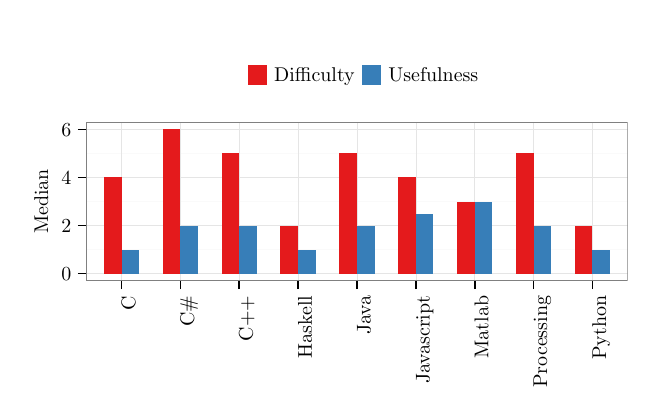
\begin{tikzpicture}[x=1pt,y=1pt]
\definecolor{fillColor}{RGB}{255,255,255}
\path[use as bounding box,fill=fillColor,fill opacity=0.00] (0,0) rectangle (216.81,130.09);
\begin{scope}
\path[clip] (  0.00,  0.00) rectangle (216.81,130.09);
\definecolor{drawColor}{RGB}{255,255,255}
\definecolor{fillColor}{RGB}{255,255,255}

\path[draw=drawColor,line width= 0.6pt,line join=round,line cap=round,fill=fillColor] ( -0.00,  0.00) rectangle (216.81,130.09);
\end{scope}
\begin{scope}
\path[clip] ( 21.16, 38.59) rectangle (216.81, 95.94);
\definecolor{fillColor}{RGB}{255,255,255}

\path[fill=fillColor] ( 21.16, 38.59) rectangle (216.81, 95.94);
\definecolor{drawColor}{gray}{0.98}

\path[draw=drawColor,line width= 0.6pt,line join=round] ( 21.16, 49.89) --
	(216.81, 49.89);

\path[draw=drawColor,line width= 0.6pt,line join=round] ( 21.16, 67.27) --
	(216.81, 67.27);

\path[draw=drawColor,line width= 0.6pt,line join=round] ( 21.16, 84.65) --
	(216.81, 84.65);
\definecolor{drawColor}{gray}{0.90}

\path[draw=drawColor,line width= 0.2pt,line join=round] ( 21.16, 41.20) --
	(216.81, 41.20);

\path[draw=drawColor,line width= 0.2pt,line join=round] ( 21.16, 58.58) --
	(216.81, 58.58);

\path[draw=drawColor,line width= 0.2pt,line join=round] ( 21.16, 75.96) --
	(216.81, 75.96);

\path[draw=drawColor,line width= 0.2pt,line join=round] ( 21.16, 93.34) --
	(216.81, 93.34);

\path[draw=drawColor,line width= 0.2pt,line join=round] ( 33.92, 38.59) --
	( 33.92, 95.94);

\path[draw=drawColor,line width= 0.2pt,line join=round] ( 55.18, 38.59) --
	( 55.18, 95.94);

\path[draw=drawColor,line width= 0.2pt,line join=round] ( 76.45, 38.59) --
	( 76.45, 95.94);

\path[draw=drawColor,line width= 0.2pt,line join=round] ( 97.72, 38.59) --
	( 97.72, 95.94);

\path[draw=drawColor,line width= 0.2pt,line join=round] (118.98, 38.59) --
	(118.98, 95.94);

\path[draw=drawColor,line width= 0.2pt,line join=round] (140.25, 38.59) --
	(140.25, 95.94);

\path[draw=drawColor,line width= 0.2pt,line join=round] (161.52, 38.59) --
	(161.52, 95.94);

\path[draw=drawColor,line width= 0.2pt,line join=round] (182.78, 38.59) --
	(182.78, 95.94);

\path[draw=drawColor,line width= 0.2pt,line join=round] (204.05, 38.59) --
	(204.05, 95.94);
\definecolor{fillColor}{RGB}{55,126,184}

\path[fill=fillColor] ( 33.92, 41.20) rectangle ( 40.30, 49.89);
\definecolor{fillColor}{RGB}{228,26,28}

\path[fill=fillColor] ( 27.54, 41.20) rectangle ( 33.92, 75.96);
\definecolor{fillColor}{RGB}{55,126,184}

\path[fill=fillColor] ( 55.18, 41.20) rectangle ( 61.56, 58.58);
\definecolor{fillColor}{RGB}{228,26,28}

\path[fill=fillColor] ( 48.80, 41.20) rectangle ( 55.18, 93.34);
\definecolor{fillColor}{RGB}{55,126,184}

\path[fill=fillColor] ( 76.45, 41.20) rectangle ( 82.83, 58.58);
\definecolor{fillColor}{RGB}{228,26,28}

\path[fill=fillColor] ( 70.07, 41.20) rectangle ( 76.45, 84.65);
\definecolor{fillColor}{RGB}{55,126,184}

\path[fill=fillColor] ( 97.72, 41.20) rectangle (104.10, 49.89);
\definecolor{fillColor}{RGB}{228,26,28}

\path[fill=fillColor] ( 91.34, 41.20) rectangle ( 97.72, 58.58);
\definecolor{fillColor}{RGB}{55,126,184}

\path[fill=fillColor] (118.98, 41.20) rectangle (125.36, 58.58);
\definecolor{fillColor}{RGB}{228,26,28}

\path[fill=fillColor] (112.60, 41.20) rectangle (118.98, 84.65);
\definecolor{fillColor}{RGB}{55,126,184}

\path[fill=fillColor] (140.25, 41.20) rectangle (146.63, 62.92);
\definecolor{fillColor}{RGB}{228,26,28}

\path[fill=fillColor] (133.87, 41.20) rectangle (140.25, 75.96);
\definecolor{fillColor}{RGB}{55,126,184}

\path[fill=fillColor] (161.52, 41.20) rectangle (167.90, 67.27);
\definecolor{fillColor}{RGB}{228,26,28}

\path[fill=fillColor] (155.14, 41.20) rectangle (161.52, 67.27);
\definecolor{fillColor}{RGB}{55,126,184}

\path[fill=fillColor] (182.78, 41.20) rectangle (189.16, 58.58);
\definecolor{fillColor}{RGB}{228,26,28}

\path[fill=fillColor] (176.40, 41.20) rectangle (182.78, 84.65);
\definecolor{fillColor}{RGB}{55,126,184}

\path[fill=fillColor] (204.05, 41.20) rectangle (210.43, 49.89);
\definecolor{fillColor}{RGB}{228,26,28}

\path[fill=fillColor] (197.67, 41.20) rectangle (204.05, 58.58);
\definecolor{drawColor}{gray}{0.50}

\path[draw=drawColor,line width= 0.6pt,line join=round,line cap=round] ( 21.16, 38.59) rectangle (216.81, 95.94);
\end{scope}
\begin{scope}
\path[clip] (  0.00,  0.00) rectangle (216.81,130.09);
\definecolor{drawColor}{RGB}{0,0,0}

\node[text=drawColor,anchor=base east,inner sep=0pt, outer sep=0pt, scale=  0.72] at ( 15.76, 38.72) {0};

\node[text=drawColor,anchor=base east,inner sep=0pt, outer sep=0pt, scale=  0.72] at ( 15.76, 56.10) {2};

\node[text=drawColor,anchor=base east,inner sep=0pt, outer sep=0pt, scale=  0.72] at ( 15.76, 73.48) {4};

\node[text=drawColor,anchor=base east,inner sep=0pt, outer sep=0pt, scale=  0.72] at ( 15.76, 90.86) {6};
\end{scope}
\begin{scope}
\path[clip] (  0.00,  0.00) rectangle (216.81,130.09);
\definecolor{drawColor}{RGB}{0,0,0}

\path[draw=drawColor,line width= 0.6pt,line join=round] ( 18.16, 41.20) --
	( 21.16, 41.20);

\path[draw=drawColor,line width= 0.6pt,line join=round] ( 18.16, 58.58) --
	( 21.16, 58.58);

\path[draw=drawColor,line width= 0.6pt,line join=round] ( 18.16, 75.96) --
	( 21.16, 75.96);

\path[draw=drawColor,line width= 0.6pt,line join=round] ( 18.16, 93.34) --
	( 21.16, 93.34);
\end{scope}
\begin{scope}
\path[clip] (  0.00,  0.00) rectangle (216.81,130.09);
\definecolor{drawColor}{RGB}{0,0,0}

\path[draw=drawColor,line width= 0.6pt,line join=round] ( 33.92, 35.59) --
	( 33.92, 38.59);

\path[draw=drawColor,line width= 0.6pt,line join=round] ( 55.18, 35.59) --
	( 55.18, 38.59);

\path[draw=drawColor,line width= 0.6pt,line join=round] ( 76.45, 35.59) --
	( 76.45, 38.59);

\path[draw=drawColor,line width= 0.6pt,line join=round] ( 97.72, 35.59) --
	( 97.72, 38.59);

\path[draw=drawColor,line width= 0.6pt,line join=round] (118.98, 35.59) --
	(118.98, 38.59);

\path[draw=drawColor,line width= 0.6pt,line join=round] (140.25, 35.59) --
	(140.25, 38.59);

\path[draw=drawColor,line width= 0.6pt,line join=round] (161.52, 35.59) --
	(161.52, 38.59);

\path[draw=drawColor,line width= 0.6pt,line join=round] (182.78, 35.59) --
	(182.78, 38.59);

\path[draw=drawColor,line width= 0.6pt,line join=round] (204.05, 35.59) --
	(204.05, 38.59);
\end{scope}
\begin{scope}
\path[clip] (  0.00,  0.00) rectangle (216.81,130.09);
\definecolor{drawColor}{RGB}{0,0,0}

\node[text=drawColor,rotate= 90.00,anchor=base east,inner sep=0pt, outer sep=0pt, scale=  0.72] at ( 38.88, 33.19) {C};

\node[text=drawColor,rotate= 90.00,anchor=base east,inner sep=0pt, outer sep=0pt, scale=  0.72] at ( 60.14, 33.19) {C\#};

\node[text=drawColor,rotate= 90.00,anchor=base east,inner sep=0pt, outer sep=0pt, scale=  0.72] at ( 81.41, 33.19) {C++};

\node[text=drawColor,rotate= 90.00,anchor=base east,inner sep=0pt, outer sep=0pt, scale=  0.72] at (102.68, 33.19) {Haskell};

\node[text=drawColor,rotate= 90.00,anchor=base east,inner sep=0pt, outer sep=0pt, scale=  0.72] at (123.94, 33.19) {Java};

\node[text=drawColor,rotate= 90.00,anchor=base east,inner sep=0pt, outer sep=0pt, scale=  0.72] at (145.21, 33.19) {Javascript};

\node[text=drawColor,rotate= 90.00,anchor=base east,inner sep=0pt, outer sep=0pt, scale=  0.72] at (166.48, 33.19) {Matlab};

\node[text=drawColor,rotate= 90.00,anchor=base east,inner sep=0pt, outer sep=0pt, scale=  0.72] at (187.74, 33.19) {Processing};

\node[text=drawColor,rotate= 90.00,anchor=base east,inner sep=0pt, outer sep=0pt, scale=  0.72] at (209.01, 33.19) {Python};
\end{scope}
\begin{scope}
\path[clip] (  0.00,  0.00) rectangle (216.81,130.09);
\definecolor{drawColor}{RGB}{0,0,0}

\node[text=drawColor,rotate= 90.00,anchor=base,inner sep=0pt, outer sep=0pt, scale=  0.72] at (  7.36, 67.27) {Median};
\end{scope}
\begin{scope}
\path[clip] (  0.00,  0.00) rectangle (216.81,130.09);
\definecolor{fillColor}{RGB}{255,255,255}

\path[fill=fillColor] ( 70.86,104.48) rectangle (167.11,121.55);
\end{scope}
\begin{scope}
\path[clip] (  0.00,  0.00) rectangle (216.81,130.09);
\definecolor{fillColor}{RGB}{228,26,28}

\path[fill=fillColor] ( 79.45,109.46) rectangle ( 86.57,116.57);
\end{scope}
\begin{scope}
\path[clip] (  0.00,  0.00) rectangle (216.81,130.09);
\definecolor{fillColor}{RGB}{55,126,184}

\path[fill=fillColor] (120.70,109.46) rectangle (127.81,116.57);
\end{scope}
\begin{scope}
\path[clip] (  0.00,  0.00) rectangle (216.81,130.09);
\definecolor{drawColor}{RGB}{0,0,0}

\node[text=drawColor,anchor=base west,inner sep=0pt, outer sep=0pt, scale=  0.72] at ( 89.08,110.53) {Difficulty};
\end{scope}
\begin{scope}
\path[clip] (  0.00,  0.00) rectangle (216.81,130.09);
\definecolor{drawColor}{RGB}{0,0,0}

\node[text=drawColor,anchor=base west,inner sep=0pt, outer sep=0pt, scale=  0.72] at (130.33,110.53) {Usefulness};
\end{scope}
\end{tikzpicture}
